\chapter{Поисковые методы идентификации}

\section{Основные понятия и параметры поисковых систем идентификации}

\subsection{Априорная и текущая информация}

Без априорной информации невозможно построение
работоспособной системы идентификации. Основные
априорные величины определяются на этапе постановки
задачи идентификации. В первую очередь это
параметры масштаба: множество допустимых
значений параметров \( \mathcal{P}\),
характерное время работы
идентифицируемой системы~$T$, а также
требуемая точность и скорость идентификации
(могут быть заданы различными способами).
В этот список может входить и ограничения на динамику изменения параметра.
В процессе работы эти параметры могут уточнятся по текущей информации.

Следующую часть априорной (по отношению к идентификации) информации
предоставляет процесс синтеза критерия идентификации.
В первую очередь, это сам вид критерия. Им определятся
как диапазон изменения величины этого критерия $\Delta q$, так и
динамические свойства:
зависимости $\sigma_q(\tau_q)$ или  $\sigma_q(a_q)$,
в простейших случаях, при заданной точности -- характерное/минимально время
оценивания \(\tau_{q,\min}\),
характерное время реакции системы $\tau_p$ на изменение
параметра с учётом динамики измерения \(q\).



\subsection{Процесс поиска}


Процесс поисковой идентификации заключается в настройке параметров одной
или нескольких моделей, определению критериев идентификации
и соответствующих функций качества, и оцениванию по этой информации
значения идентифицируемого параметра $p_{id}$.
При использовании в целях идентификации нескольких моделей,
появляются общие действия, применяемые к каждой из них.

\section{Структура поисковых систем}

\section{Свойства, параметры и классификация поисковых агентов}

Введём необходимые для дальнейшего изложения определения.

Определение: \textbf{поисковый агент} -- это динамическая система, получающая выходной ($x(t)$),
и, при необходимости входной сигнал ($u(t)$) от одной или нескольких моделей,
величину критерия качества, определённую для объекта $q_o(t)$,
может быть информацию от других поисковых агентов,
на основании значения критерия идентификации
реализующая алгоритм настройки параметра модели (моделей)
таким образом, чтобы обеспечить идентификацию заданного параметра.

Один поисковый агент может управлять как одной моделью (рис.~\ref{atu:f:agent1}, \ref{atu:f:agent1q}),
так и несколькими (рис.~\ref{atu:f:agent2}).
При этом он может использовать информацию,
как полученную непосредственно от других агентов,
так и вычисленную в результате обработки данных на других уровнях системы идентификации.

Основным выходным сигналом агента будем считать текущее
значение его параметра $p_i(t)$. Дополнительными,
но нем не менее значимыми величинами является
$F_i(t)$ -- текущее значение функции качества
(если используется одна  модель для агента, или же если агент каким-либо образом её усредняет
или аппроксимирует в случае нескольких моделей),
$q_i(t)$ -- значение критерия качества (аналогично предыдущей величине в случен нескольких моделей),
$p_e(t)$ -- оценка идентифицируемого параметра текущим агентом.


\textbf{ Рой } -- множество агентов, обеспечивающее идентификацию за счёт
сосредоточения максимального количества агентов
в области предполагаемого максимума функции качества.
Обычно -- три составляющие поведения
(движение о оцениваемому локальному экстремуму, -- к глобальному, случайная составляющая).

\Cmt{Для сравнения требуется и это промоделировать.
Достаточно накладно -- надо много агентов.}

Достоинства -- простота алгоритмов.
Недостатки -- требуется избыточное количество агентов.
Значительная часть агентов, находящихся вблизи экстремума,
практически не приносит информации. Роевые
алгоритмы (как и их прообразы в живой природе) ориентированы
для увеличения добычи ресурсов, а не информации. % TODO: link

\textbf{ Ансамбль } -- множество агентов, обеспечивающее идентификацию за счёт
распределения агентов таким образом, который обеспечивает как
точность идентификации за счёт ограниченного скопления агентов
в областях предполагаемых максимумов, так и оперативное переключение
на другие области при изменении параметров за счёт недопущения
неоправданной скученности агентов.


\begin{figure}[htb!]
\begin{center}
% vi:syntax=tex
\begin{tikzpicture}
  \bXStyleBloc{semiboldline,inner sep=2pt};
  \bXLineStyle{medline};
  % --- U
  \bXInput{U};
  % --- M
  \bXBlocL[2.0]{M}{$\mathbf{M}_i$}{U};
  \bXLink[$u(t)$]{U}{M};
  % --- Q
  \bXBloc[3.5]{Q}{$q(t)$}{M};
  \path (Q.east) ++(0.0,-1.0em) coordinate (Qqm);
  \path (Q.south west) ++(-0.3,-0.4) coordinate (BLKlb);
  \bXLink[$x_i(t)$]{M}{Q};
  % --- F
  \bXBloc[2.5]{F}{$F(q_o,q_{mi})$}{Q};
  \path (F.west) ++(0.0,-1.0em) coordinate (Fqm);
  \path (F.west) ++(0.0,+1.0em) coordinate (Fqo);
  \path (Fqo) ++(-1.6em,+2.8em) coordinate (Fqoi) {};  % external input
  \draw[medlinep] (Fqoi) |- (Fqo);
  \node[below right] at (Fqoi) {$q_o(t)$};
  \bXLink[$q_i(t)$]{Qqm}{Fqm};
  % --- P
  \bXBloc[2]{P}{$P$}{F};
  \draw[boldline,<->] (P.north) -- +(0,0.8);
  \path (P.north east) ++(0.1,+0.4) node (BLKrt) {};
  \bXLink[$F_i(t)$]{F}{P};
  % -- output
  \bXOutput[2.8]{Po}{P};
  \bXLink[$p_i(t)$]{P}{Po};
  \bXOutput[1.0]{Por}{P};
  \fill(Por) circle[radius=0.05];
  \bXLineStyle{semiboldline};
  \bXReturn{Por}{M}{$p_i(t)$};
  % -- block
  \draw[subelem] (BLKlb) |- (BLKrt) |- (BLKlb);
  \bXStyleBlocDefault;
  \bXDefaultLineStyle;
  %
  \TikzAddPadding
  %
\end{tikzpicture}

\end{center}
\caption{Поисковый агент, использующий функцию качества $F$, и настраивающий параметр одной модели}
\label{atu:f:agent1}
\end{figure}


\begin{figure}[htb!]
\begin{center}
% vi:syntax=tex
\begin{tikzpicture}
  \bXStyleBloc{semiboldline,inner sep=2pt};
  \bXLineStyle{medline};
  % --- U
  \bXInput{U};
  % --- M
  \bXBlocL[2.0]{M}{$\mathbf{M}_i$}{U};
  \bXLink[$u(t)$]{U}{M};
  % --- Q
  \bXBloc[3.5]{Q}{$q$}{M};
  \path (Q.east) ++(0.0,-1.0em) coordinate (Qqm);
  \path (Q.south west) ++(-0.3,-0.4) coordinate (BLKlb);
  \bXLink[$x_i(t)$]{M}{Q};
  % --- P
  \bXBloc[2]{P}{$P$}{Q};
  \draw[infoline,<->] (P.north) -- +(0,0.8);
  \path (P.west) ++(0.0,-1.0em) coordinate (Pqm);
  \path (P.west) ++(0.0,+1.0em) coordinate (Pqo);
  \path (Pqo) ++(-1.6em,+2.8em) coordinate (Pqoi) {};  % external input
  \path (P.north east) ++(0.1,+0.4) node (BLKrt) {};
  \bXLink[$q_{i}(t)$]{Qqm}{Pqm};
  \draw[medlinep] (Pqoi) |- (Pqo);
  \node[below right] at (Pqoi) {$q_o(t) \qquad A_i$};
  %\bXLink[$F_i(t)$]{F}{P};
  % -- output
  \bXOutput[2.8]{Po}{P};
  \bXLink[$p_i(t)$]{P}{Po};
  \bXOutput[1.0]{Por}{P};
  \fill(Por) circle[radius=0.05];
  \bXLineStyle{semiboldline};
  \bXReturn{Por}{M}{$p_i(t)$};
  % -- block
  \draw[subelem] (BLKlb) |- (BLKrt) |- (BLKlb);
  \bXStyleBlocDefault;
  \bXDefaultLineStyle;
  %
  \TikzAddPadding
  %
\end{tikzpicture}

\end{center}
\caption{Поисковый агент, использующий критерий $q$, и настраивающий параметр одной модели}
\label{atu:f:agent1q}
\end{figure}


В случае, когда один агент настраивает несколько моделей,
или/и, если пространство параметров имеет размерность больше единицы,
вместо простого индекса $i$ могут применяется составные.

\begin{figure}[htb!]
\begin{center}
% vi:syntax=tex
\begin{tikzpicture}
  %\draw[hair,step=1.0em] (0,-3) grid (12.0,3.0);
  \bXStyleBloc{semiboldline,inner sep=2pt};
  \bXLineStyle{medline};
  % --- U
  \bXInput{U};
  \path (U.center) ++(2.5em,0.0em) coordinate (UxM);
  \draw (U.center) -- (UxM);
  \fill (UxM) circle[radius=0.05];
  \node[above right] at(U) {$u(t)$};
  % --- M0
  \bXBranchy[2]{UxM}{U0};
  %\fill[red](U0) circle[radius=0.05];
  \bXBlocL[2.0]{M0}{$\mathbf{M}_{i0}$}{U0};
  \bXLinkyx{UxM}{M0};
  % --- M1
  \bXBranchy[-2]{UxM}{U1};
  %\fill[green](U1) circle[radius=0.05];
  \bXBlocL[2.0]{M1}{$\mathbf{M}_{i1}$}{U1};
  \bXLinkyx{UxM}{M1};
  % --- A
  \path (M0.east) ++(3.1em,0.0em) coordinate (X0);
  \path (X0) ++(4.0em,0.0em) coordinate (P0S);
  \path (X0) ++(0.0em,-2.0em) coordinate (Alb);
  %\fill[red](Alb) circle[radius=0.05];
  \path (M1.east) ++(3.1em,0.0em) coordinate (X1);
  \path (X1) ++(4.0em,0.0em) coordinate (P1S);
  \path (X1) ++(0.0em,2.0em) coordinate (Alt);
  \path ( $0.5*(P0S) + 0.5*(P1S)$ ) coordinate(PS);
  \path ( $0.5*(X0) + 0.5*(X1)$ ) coordinate(QO);
  \draw[medlinep] (QO) ++(-3.2em,0em) -- (QO);
  \node[above left] at(QO) {$q_{o}(t)$};
  %\fill[green](Alt) circle[radius=0.05];
  \draw[boldline] (Alb) -- ++(4.0em,0.0em) |- (Alt) -- cycle; % ----- MAIN block
  \draw[medlinep] (M0.east) -- (X0); // % inputs: x_ix(t)
  \node[above right] at(M0.east) {$x_{i0}(t)$};
  \draw[medlinep] (M1.east) -- (X1);
  \node[above right] at(M1.east) {$x_{i1}(t)$};
  \draw[semiboldlinep] (P0S) -- ++(3.0em,0em) -- ++(0em,-3.0em) -| (M0.south); % -- out params
  \node[above right] at(P0S) {$p_{i0}(t)$};
  \draw[semiboldlinep] (P1S) -- ++(3.0em,0em) -- ++(0em,+3.0em) -| (M1.north);
  \node[above right] at(P1S) {$p_{i1}(t)$};
  \draw[medlinep] (PS) -- ++(4.0em,0em);
  \node[above right] at(PS) {$p_{i}(t)$};
  \path (PS) ++(-2.1em,0.0em) coordinate (AI);
  \node at(AI) {$\mathbf{A}_{i}$};
  %
  \TikzAddPadding
  %
\end{tikzpicture}

\end{center}
\caption{Поисковый агент, настраивающий параметры двух моделей}
\label{atu:f:agent2}
\end{figure}

\begin{figure}[htb!]
\begin{center}
../../p3/p/agents.pgf
\end{center}
\caption{Мультиагентная система идентификации с плоской структурой}
\label{atu:f:agents}
\end{figure}

\subsection{Один агент}

Единственный неподвижный агент практически не имеет смысла
с точки зрения синтеза системы идентификации.
Он может сигнализировать о том, что в пределах
\(\tau\) модель была или не была достаточно адекватна
объекту.

Наличие истории и возможность перемещаться дают возможность
построить систему идентификации и на одном агенте.
В качестве истории могут использоваться, в том числе,
динамические свойства идентифицируемого объекта
(оригинальный метод АПИ). Также могут быть
применены интегрирующие элементы агента идентификации
(синхронный детектор, \ldots).

В простейших случаях возможно построение системы идентификации
с одной моделью и, соответственно, одним поисковым агентом.
Примерами такого похода могут служить
метод синхронного детектора \cite{adopt_cont_sys}
и оригинальный адаптивно-поисковый метод \cite{mich_92}.
Применение одномодельных методов требует определённого механизма
сохранения истории процесса поиска, по крайней мере в пределах
одного поискового ``периода''. Это сильно ограничивает диапазон
применимости данных методов, в первую очередь -- из-за значительных
временных затрат на повторяющийся поиск.

Применение пары моделей \cite{atu_asau3}
(в этом случае имеет смысл говорить об одном поисковом агенте)
позволяет с меньшими временными затратами оценить градиент функции качества,
и, как следствие -- определить значение параметра. Также значительным плюсом
такого подхода является меньшая скорость изменения параметров моделей.


Пара агентов, взаимодействующая между собой,
способна оценить градиент функции качества,
и, следовательно, обеспечить смещение в требуемом направлении.

С учетом глобальной информации возможна адаптация параметров пары.
В свою очередь, информация, полученная от пары может
использоваться для уточнения глобальных параметров.


Тем не менее, при использовании пары моделей неоправданно много времени
тратится на перемещение поисковой пары, особенно при резких изменениях
идентифицируемого параметра. Поэтому, использование множества
поисковых агентов может кардинально уменьшить время идентификации.

\subsubsection{Пара агентов}

Каждый поисковый агент, определяя величину $q_{i}(t)$ , и получая $q_o(t)$,
вычисляет безразмерную функцию качества идентификации
$F(q_o,q_i)$.

С учётом обозначения
%
\[
  q_r = \frac{q_o - q_m}{q_\gamma},
\]
%
\noindent
представлены наиболее распространённые виды таких функций~\cite{atu_ISDMCI2016}:
%
\begin{equation}
  F_{\mathrm{gauss}} = \exp( - q_r^2 ),
\label{atu:eq:F_gauss}
\end{equation}
%
\begin{equation}
  F_{\mathrm{parabolic}} = 1 - q_r^2 \left( 1 - \frac{1}{e} \right),
\label{atu:eq:F_parabolic}
\end{equation}
%
\begin{equation}
  F_{\mathrm{triangle}} = 1 - |q_r| \left( 1 - \frac{1}{e} \right),
\label{atu:eq:F_triangle}
\end{equation}
%
\begin{equation}
  F_{\mathrm{hyper}} = \frac{1}{ 1 + |q_r| \left( 1 - \frac{1}{e} \right)},
\label{atu:eq:F_hyper}
\end{equation}
%
\begin{equation}
  F_{\mathrm{log}} = 1 - \ln \left( 1 + |q_r| \right) \frac{1-1/e}{\ln(2)}.
\label{atu:eq:F_log}
\end{equation}

Для всех рассмотренных функций $q_\gamma$ -- величина, обратная чувствительности
функции качества, задаёт масштаб и рабочий диапазон функции качества (рис.~\ref{atu:f:F_types}).
При этом, при необходимости, значения этих функций могут быть искусственно ограничены диапазоном $[0;1]$.
Каждая имеет свой набор преимуществ и недостатков~\cite{atu_ISDMCI2016}.
Подробнее этот вопрос будет рассмотрен в главе~\ref{atu:ch:testsys}.

\begin{figure}[htb!]
  \centerline{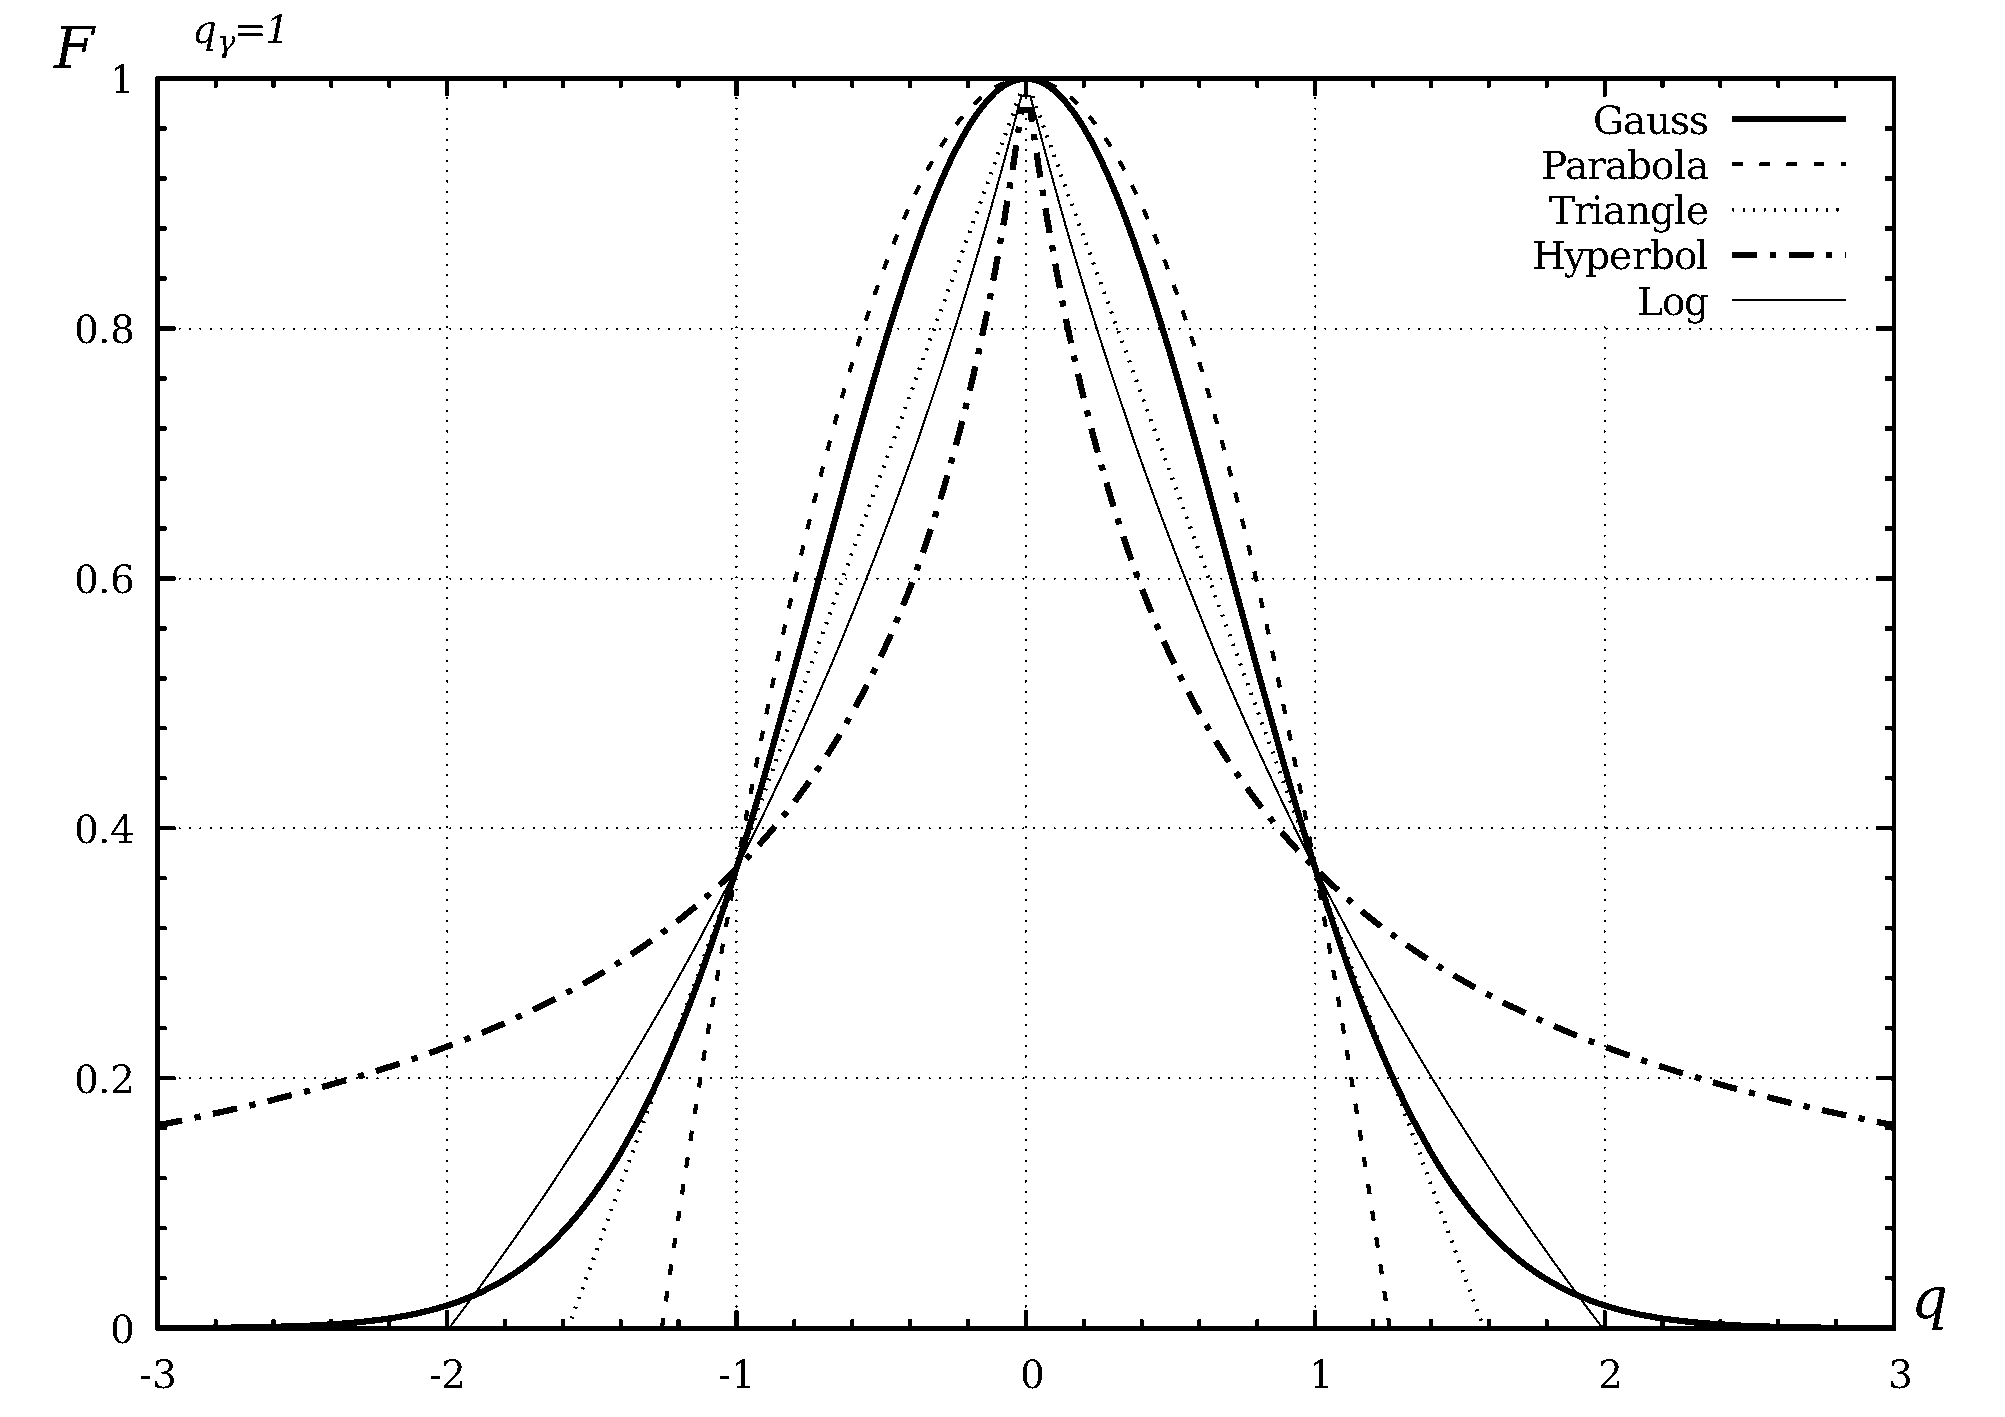
\includegraphics[width=45\TW]{p/F_types.png} }
  \caption{Функции качества идентификации (\ref{atu:eq:F_gauss})--(\ref{atu:eq:F_log})}
  \label{atu:f:F_types}
\end{figure}

\subsubsection{Триплет агентов}

Рассмотрим случай, когда каждый агент взаимодействует с двумя своими ближайшими соседями,
запрашивая у них величины $p$ -- текущее значение параметра и $F$.
При анализе конкретного агента, для упрощения записи, его индекс $i$ обозначим как ``c'' (current),
предыдущий получает индекс ``l'' (left), а последующий -- ``r'' (right).
Для единообразия дополним множество моделей двумя неподвижными псевдомоделями (fake models),
обозначив их индексами ``ll'' и ``rr''. Для псевдомоделей считаем $  F_{ll} = F_{rr} = 0$,
а координаты выбираются за пределами рабочего диапазона поиска.



Три соседних агента, взаимодействующие между собой,
способны не только оценить градиент функции качества в своей окрестности,
но и определить (опять же, оценочно) наличие там максимума.

\paragraph{Идеальный случай}

Пусть зависимость $q(p)$ задана самым простым и благоприятным для идентификации способом:
%
\[
  q(p) = p_0 + b_p p .
\]
Шумы измерения и прочие помехи отсутствуют.
Рассмотрим 3 соседних поисковых агента: $A_l$, $A_c$, $A_r$.
Тогда, если $p_o \in [ p_l, p_r ] $, оценка положения
идентифицируемого параметра $p_e$, выполненная агентом $A_c$,
должна совпадать с реальным значением параметра объекта: $p_e = p_o $.
Если $p_o \notin [ p_l, p_r ] $, то конкретное расположение
$p_e$ значения не имеет, достаточно потребовать определения направления
этого расположения относительно диапазона. % TODO: и может быть чего-то ещё для адаптации


% TODO: full rewrite,
\begin{figure}[htb!]
  \centerline{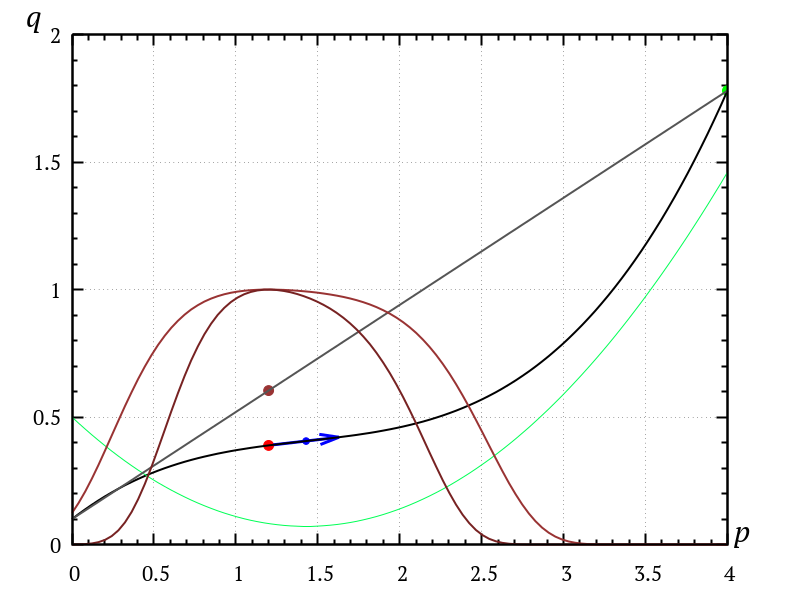
\includegraphics[width=0.6\textwidth]{pq_1x2.png} }
  \caption{ $q(p)$, $F(q(p))$, part1 }
  \label{atu:pq_1x2}
\end{figure}

\begin{figure}[htb!]
  \centerline{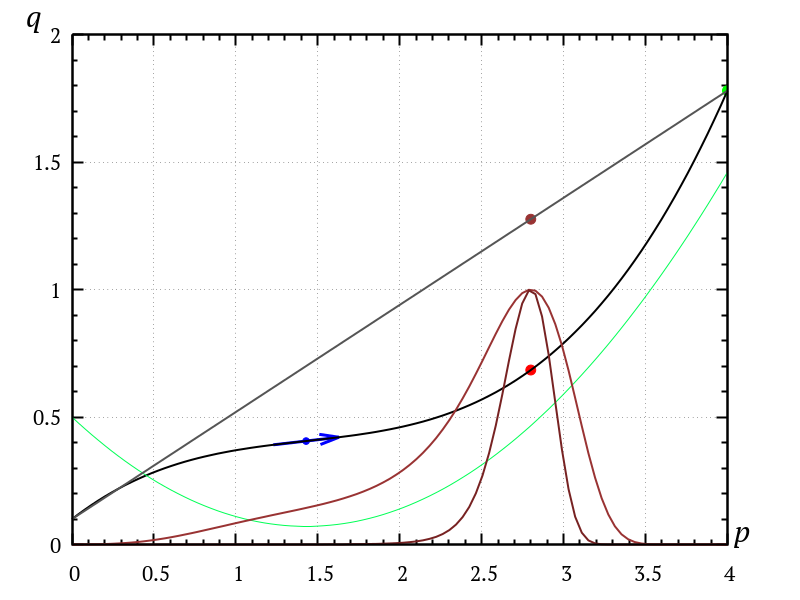
\includegraphics[width=0.6\textwidth]{pq_2x8.png} }
  \caption{$q(p)$, $F(q(p))$, part2 }
  \label{atu:pq_2x8}
\end{figure}

\subsubsection{Ансамбль агентов}


\subsection{Время и история}

Способы учёта истории системы и динамических характеристик.

Явное представление истории -- каждый агент имеет способ хранения и использования
информации о предыдущих значениях параметра и критерия.

Неявное представление истории -- тот факт, что в данный момент времени известно
текущее значение параметра и критерия, с учетом известных значений
параметров поиска самого агента, может неявно дать ограниченную информацию
о предыдущем состоянии.

Стабильные/мобильные модели.

История: локальная + глобальная




Рассмотрим 3 подхода к определению
точки максимума функции качества, а следовательно -- значения идентифицируемого параметра \cite{atu_st99,atu_jacs2015}.
Первый -- реализация
метода COG (Center of gravity, Такаги-Сугено) \cite{atu_asau25,atu_csit2015},
используемого при дефаззификации систем нечёткой логики:
%
\begin{equation}
  p_{ge}
  =
  \frac{\sum\limits_{i=0}^{n-1} F_{i} p_{i}}
       {\sum\limits_{i=0}^{n-1} F_{i} }
  .
  \label{atu:eq:p_ge}
\end{equation}

Второй подход призван уменьшить зависимость первого
от влияния локальных экстремумов и границ. В этом
случае определяется модель $M_{i_{m}}$ с максимальным значением
$F$, а в оценке используется только ближайшая окрестность этой модели:
%
\begin{equation}
  p_{le}
  =
  \frac{ F_{i-1} p_{i-1} + F_{i} p_{i} + F_{i+1} p_{i+1} }
       { F_{i-1}         + F_{i}       + F_{i+1}         }
  ;
  \quad
  i : F_i = \max{F_j}, \, j=0 \ldots n-1.
  \label{atu:eq:p_le}
\end{equation}
%
или, у учётом введённых локальных обозначений:
%
\begin{equation}
  p_{le}
  =
  \frac{ F_{l} p_{l} + F_{c} p_{c} + F_{r} p_{r} }
       { F_{l}       + F_{c}       + F_{r}       }
  .
  \label{atu:eq:p_lel}
\end{equation}

Третий подход отличается от второго тем, что по трём точкам вблизи  $M_{i}$
функция $F(p)$ аппроксимируется параболой, и абсцисса её вершины задаёт искомое
значение параметра. Сместим начало координат в точку
$ ( p_c, F_c ) $. Тогда
%
\[
  \tilde{p}_c = 0, \,
  \tilde{p}_l = p_l - p_c, \,
  \tilde{p}_r = p_r - p_c.
\]
%
\[
  \tilde{F}_c = 0, \,
  \tilde{F}_l = F_l - F_c, \,
  \tilde{F}_r = F_r - F_c.
\]
%
\[
  \left\{
    \begin{array}{l}
      a_2 \tilde{p}_l^2 + a_1 \tilde{p}_l  = \tilde{F}_l
      \\
      a_2 \tilde{p}_r^2 + a_1 \tilde{p}_r  = \tilde{F}_r
    \end{array}
  \right. .
\]
%
\[
  a_1 = \frac{\tilde{F}_r \tilde{p}_l^2 - \tilde{F}_l \tilde{p}_r^2 }
             { \tilde{p}_l^2 \tilde{p}_r  + \tilde{p}_l \tilde{p}_r^2 }.
\]
%
\[
  a_2 = \frac{\tilde{F}_r \tilde{p}_l - \tilde{F}_l \tilde{p}_r }
             { \tilde{p}_l^2 \tilde{p}_r  + \tilde{p}_l \tilde{p}_r^2 }.
\]

\begin{equation}
  \tilde{p}_e = - \frac{a_1}{2 a_2};
  \;
  p_e = p_c -- \frac{a_1}{2 a_2}.
  \label{atu:eq:p_e}
\end{equation}


При этом, если
$ p_e \notin [ p_l, p_r ] $, или $ a_2 \ge 0 $, то значение $p_e$ искусственно
ограничивается этим диапазоном. Значение $p_e$ для модели с индексом
$i_m$ обозначим как $p_{ee}$ и будем считать
текущим значением идентифицируемого параметра, полученным с помощью
третьего подхода. Ошибки идентификации в пространстве параметров
для рассмотренных трёх подходов обозначим соответственно:
%
\begin{equation}
  e_{ge} = p_{ge} - p_o, \;
  e_{le} = p_{le} - p_o, \;
  e_{ee} = p_{ee} - p_o.
  \label{atu:eq:e_xx}
\end{equation}


Динамика изменения параметров моделей (поисковых агентов) задаётся следующим образом:
%
\begin{equation}
  \od{p_c}{t} = v_f f_t(t),
  \label{atu:eq:dp_dt}
\end{equation}
%
\noindent
где $f_t$ -- сумма всех действующих ``сил'', $v_f$ -- коэффициент
пропорциональности. Рассмотрим 3 действующие силы
($ f_t = f_c + f_n + f_e $):

\begin{enumerate}
  \item
    $f_c = -k_c (p_c - p_{c,0}) $ -- ``сила притяжения'' к начальному значению
    параметра
    для данной модели. Наличие этой силы не даёт всем моделям принять одно
    и то же значение параметра вблизи экстремума, и, следовательно,
    прекратить процесс поиска. Это также позволяет быстро переключиться
    на другую модель в случае быстрого изменения параметра объекта.

  \item
    $f_n = k_n ( p_r - 2 p_c + p_l ) $ -- ``сила взаимодействия''
    с соседями. Обеспечивает более равномерное распределение
    параметров моделей вблизи экстремума.

  \item
    $f_e = - k_e ( p_c - p_e ) $ -- ``сила притяжения'' к локальной
    оценке экстремума, определённого по выражению~(\ref{atu:eq:p_e}).

\end{enumerate}

Результаты моделирования показали, что в некоторых случаях
имеет смысл введение дополнительных сил ``барьерного'' вида,
для исключения пересечения траекторий поисковых агентов, или же их ухода из рабочего диапазона.






\section{Классификация и обозначения систем идентификации}
\label{atu:id_classification}

В данной работе рассматривается набор методов идентификации нелинейных динамических
систем. При этом, большинство из них имеют общие свойства, и система идентификации в  целом
состоит из ``набора'' модулей и алгоритмов, комбинация которых
позволяют выбрать конкретный метод, подходящий для данной задачи.
Следовательно, возникает вопрос корректного и непротиворечивого обозначения
используемого метода. Ввиду значительного количества методов, полученных
путём комбинации их элементов, не имеет смысла давать каждому
отдельное названия. Возникает потребность в унификации обозначений
методов, и соответственно, введения определённой классификации.

Предлагается к использованию следующая система обозначений:

\begin{enumerate}

  \item  Первый символ определяет, какая величина ($q$ или $F$) используется
    каждым агентом для определения $p_e$. Соответственно, первый символ
    будет ``q'' или ``F''.
    Для обозначения методов, для которых в качестве критерия используется
    непосредственно выходы моделей и объектов, использует символ ``x''.
    При необходимости, при появлении новых подходов,
    могут быть назначены дополнительные символы.

  \item
    Второй символ задаёт способ определения идентифицируемого параметра по всему ансамблю:
    \begin{description}

      \item[b]  -- ``best'' -- выбирается лучший агент без дальнейшей обработки;

      \item[g]  -- ``global COG'' -- метод ``Center of Gravity'' по всему ансамблю~(\ref{atu:eq:p_ge});

      \item[l] -- ``local COG'' --   метод ``Center of Gravity'' по окрестности лучшего агента~(\ref{atu:eq:p_le});

      \item[e] -- квадратическая интерполяция по $F$ в окрестности лучшего агента~(\ref{atu:eq:p_e});

      \item[x] -- ``extremum COG'' -- вариант ``Center of Gravity'' по всему ансамблю, при этом
        от каждого агента используются величины $p_e$ и $FS_e$.

    \end{description}

    В случае, если вместо ансамбля используется 1--2 агента, то для определённости будет
    использован символ ``b''

  \item
    Третий символ обозначает выбранную зависимость для величины $f_e$:
    \begin{description}

      \item[c]  -- ``const'' -- величина $f_e$ не участвует в описании
        динамики поискового агента;

      \item[l] -- ``linear'' --  величина $f_e$ линейно зависит
        от $p_e$: $f_e = k_e ( p_e - p_c )$;

      \item[s] -- ``sign'' -- используется зависимость вида
        от $p_e$: $f_e = k_e \sign( p_e - p_c )$;

      \item[u] -- ``saturate'' -- аналогично ``s'', но используется небольшой
        линейный участок при $p_e \approx p_c$.

    \end{description}


  \item
    Четвёртый символ указывает, каким образом величина $f_t$ влияет на динамику агента:
    \begin{description}

      \item[z]  -- ``zero'' -- агент неподвижен;

      \item[v] -- ``viscous'' --  используется модель вязкого трения; % TODO: ref;

      \item[b] -- ``ball'' -- используется подход ``тяжёлого шарика'';

      \item[s] -- ``special'' -- особый вид, задаётся методом непосредственно.

    \end{description}

  \item
    Пятый символ позволяет указать, какое дополнительное поисковое движение
    реализует агент
    \begin{description}

      \item[n]  -- ``none'' -- дополнительное поисковое движение не используется,
        при этом, если не возникает неоднозначности в классификации, данный символ можно упустить;

      \item[t] -- ``triangle'' --  используется пилообразное поисковое движение, например, реализуемое
        с помощью УГПК; % TODO: ref;

      \item[d] -- ``dual'' -- используется поисковое движение, реализуемое парой УГПК;

      \item[s] -- ``sin'' --  используется гармоническое поисковое движение;

      \item[r] -- ``random'' --  используется случайное поисковое движение.

    \end{description}

  \item
    Следующая группа символов указывает количество активных агентов.
    В одномерном случае это или просто число, или символ ``N'', если
    конкретное количество несущественно. В двумерном случае
    используются варианты ``NxM'' для сеточного расположения агентов,
    и ``NpM'  -- для конфигурации ``крест''. В случае большей размерности
    пространства параметров можно использовать аналогичные обозначения,
    но, при необходимости, с дополнительными индексами, например:
    ``10x10p5'', ``$\mathrm{N_1 p N_2 x N_3 p N_4}$''.

  \item
    Следующий символ, записанный после символа ``.'' указывает количество агентов в
    в поисковой группе, например: ``2'' -- поисковая пара, ``3'' -- триплет.

  \item Восьмой символ, указываемый при необходимости, описывает
    поведение дополнительных моделей, находящихся на границе:
    \begin{description}

      \item[z]  -- ``zero'' -- реальная модель не используется, функция качества $F$ для неё считается нулевой;

      \item[к] -- ``real'' --  используется реальная модель, но без возможности её смещения;

      \item[а] -- ``approximate'' -- значение критерия и функции качества каким-то образом аппроксимируются;

    \end{description}

\end{enumerate}

При необходимости, в конец данного обозначения, через точку, добавляется обозначение используемого критерия.
Дополнительное компоненты добавляются в конец после двоеточия. Для обозначения подмножеств методов
вместо обозначения элемента используется символ ``A'' -- ``any''.


Примеры обозначений:

``Fglv5.3z.$q_{x^2}$'' -- метод, использующий 5 подвижных (3 триплета) и 2 ``fake'' модели,
``global COG'' для результирующего значения параметра
для оценивания величины $p_e$ используется функция качества,
зависимость $f_e$ от $p_e$ -- линейная, ``вязкая'' динамика, критерий ``$q_{x^2}$''.


``qAuv7.3r.$q_{dx}$'' -- методы, использующий 7 подвижных (5 триплетов) и 2 ``real'' модели на границах,
для оценивания величины $p_e$ используется значение критерия,
зависимость $f_e$ от $p_e$ -- с насыщением, ``вязкая'' динамика, критерий ``$q_{dx}$'',
используются все доступные методы для определения  результирующего значения параметра.

``xblst1'' -- оригинальный адаптивно-поисковый метод.

``xblsd2.2'' -- адаптивно-поисковый метод с двумя моделями и двумя УГПК с общим сбросом.

``Fgcz7x7.1'' -- сетка из 49 ($7 \times 7$) неподвижных моделей,
``global COG'' для результирующего значения параметра,
без указания конкретного критерия.

\section{Адаптация}

Какие параметры системы идентификации можно адаптировать
и на каком уровне.

Когда имеет смысл играть с чувствительностью.

% Как близко имеет смысл подводить модели к экстремуму?

\section{Качество идентификации}

Среди множества способов оценивания качества идентификации
можно выделить две группы.
К первой группе относятся те, которые производят оценивание
только на основе критерия идентификации, или,
что в какой-то мере эквивалентно, по функции качества идентификации.
В реальных задачах, когда нет возможности определить реальные значения
параметров объекта, это практически единственный вариант.
При этом подразумевается, что как критерий идентификации, так и
функция качества выбраны корректно.

В процессе синтеза новых критериев и методов идентификации
такой подход, с одной стороны, слишком строг,
с другой -- не даёт проверить корректность полученного результата,
так как в этом случае ни близость критериев модели и объекта,
ни, тем более, близкое к единице значение функции качества не
обозначает работоспособность системы идентификации.
Следовательно, при анализе работоспособности,
которые проводятся как на модельных задачах,
так и на реальных физических объектах в контролируемых
условиях, необходимо использовать методы из второй группы,
основанные на сравнении собственно параметров модели и объекта,
то есть на оценивании параметрической
ошибки идентификации $e(t)=p_o(t)-p_{id}(t)$.

В работах [citkin,myPphd,xxx] были предложены информационные методы
оценивания качества идентификации.
Они отличаются универсальностью, и отображают
успешность решения одной из основных задач
идентификации -- получения информации то объектах.
Однако, для построения информационных оценок
требуется значительно больше ресурсов, чем
для проведения собственно идентификации. В некоторых случаях,
например, при получении данных с реального оборудования,
это может быть просто невозможно.



При таких условиях, качество идентификации для процесса
в целом задаётся мерой:
%
\[
  \overline{e} = \mu( p_o(t), p_{id}(t) ),
  \quad
  t \in [0;T].
\]

Конкретный вид меры определяется задачей.
Если в конкретной постановке важно знать максимальное
отклонение идентифицируемого параметра модели от объекта,
то имеет смысл выбрать меру $C[0;T]$~\cite{kolmogorov_fun_ana} или же
$R_{\infty}^n$ для дискретного представления:
%
\begin{equation}
  \overline{e_c}(p_o(t),p_{id}(t))
  =
  \max \big| p_o(t)-p_{id}(t) \big|,
  \quad
  t \in [0;T].
  \label{atu:eq:e_c}
\end{equation}

Более распространённым является случай,
когда интерес представляет не максимальное значение $|e(t)|$,
а какой-то вариант усреднения этой величины, например
%
\begin{equation}
  \overline{e_2}(p_o(t),p_{id}(t))
  =
  \sqrt{ \frac{1}{T} \int\limits_{0}^{T} \big( p_o(t)-p_{id}(t) \big)^2 \, \mathrm{d}t },
  \label{atu:eq:e_2}
\end{equation}
%
или
\begin{equation}
  \overline{e_1}(p_o(t),p_{id}(t))
  =
  \frac{1}{T} \int\limits_{0}^{T} \big| p_o(t)-p_{id}(t) \big| \, \mathrm{d}t .
  \label{atu:eq:e_1}
\end{equation}
%
Этот подход особенно оправдан в тех случаях, когда
значение параметра объекта претерпевает резкие изменения.
При этом, никакая система идентификации не будет успевать за такими
изменениями, особенно с учётом времени, необходимого для
оценивания критерия. Следовательно, если оценивать в таких условиях
качество идентификации, используя \ref{atu:eq:e_c},
то в качестве результата получим всего лишь величину
скачков параметра, а не какие-либо характеристики процесса идентификации.

В тех, достаточно редких случаях, когда из априорной
информации о системе известно, что $p_o(t) = \mathrm{const}$,
имеет смысл в выражениях~(\ref{atu:eq:e_c})--~(\ref{atu:eq:e_1})
ограничить диапазоны для времени, например $[T-\tau_p,T]$,
где $\tau_p$ -- время, достаточное для измерения
критерия идентификации с требуемой точностью.
Это позволит избежать влияния переходных процессов
идентификации на интегральную оценку ошибки.
В остальных случаях, представляет интерес именно реакция
на изменения параметра, поэтому в данной работе преимущественно будет
использоваться выражение~(\ref{atu:eq:e_2}).




Само значение как ошибки идентификации, так и соответствующей меры -- величина размерная,
и в таком виде не пригодно для
независимого от конкретной ситуации оценивания качества работы метода.
Рассмотрим возможные величины, дающие возможность обезразмерить ошибку идентификации.

В первую очередь, предположим, что вообще не проводим никакой идентификации,
а в качестве значения параметра используем или геометрический центр $p_{00}$ множества $\mathcal{P}$,
или, если это по какой-либо причине известно, точку с максимальным значением плотности вероятности.
Тогда обозначим
%
\begin{equation}
  \overline{e}_{00}
  =
  \overline{e}(p_o(t),p_{00})
  \label{atu:eq:e_00}
\end{equation}

Относительные ошибки для соответствующих абсолютных~(\ref{atu:eq:e_xx})
тогда будут определены следующим образом:
%
\begin{equation}
  \overline{e}_{rge} = \frac{\overline{e}_{ge}}{\overline{e}_{00}}, \;
  \overline{e}_{rle} = \frac{\overline{e}_{le}}{\overline{e}_{00}}, \;
  \overline{e}_{xee} = \frac{\overline{e}_{xe}}{\overline{e}_{00}}, \;
  \overline{e}_{ree} = \frac{\overline{e}_{ee}}{\overline{e}_{00}}.
  \label{atu:eq:e_rxx}
\end{equation}

Близость этих величин к единице свидетельствует о том, что
данный метод идентификации в рассматриваемых условиях бесполезен.
Более того, при серьёзных нарушениях в процессе поиска,
например при потере устойчивости, эти величины могут и превосходить единицу.

Несмотря на очевидную пользу, такой способ приведения к безразмерному виду ошибок
имеет ряд недостатков. Во-первых,
не учитывается возможная мультиагентная структура системы идентификации,
для которой оценка ~(\ref{atu:eq:e_00}) будет слишком грубой.
С другой стороны,
не учитываются свойства
самой системы. Например, возможна такая ситуация, когда параметр
объекта изменяется настолько быстро (по отношению к времени оценивания критерия),
что любой метод идентификации будет бесполезен.

Для оценивания качества работы системы идентификации с счётом
множества моделей, можно воспользоваться несколькими приёмами.
Первый -- пусть все агенты неподвижны, а в качестве $p_{id}(t)$
используется $p_c$ той модели, функция качества для которой
максимальна. Обозначим полученное таким образом значение
параметра как $p_{bm}(t)$ (``best model''),
соответствующую ему усреднённую ошибку как $\overline{e}_{bm}$.
При этом безразмерные величины обозначим как
$\overline{e}_{bmge}$, $\overline{e}_{bmle}$,  \ldots.
Близость этих величин к единице, при одновременной малости
$\overline{e}_{r*}$, свидетельствует о том, что передвижения
агентов практически бесполезны, и работоспособность системы идентификации достигается
практически только за счёт переключения между агентами.
Одной из причин такого поведения, при условии отсутствия ошибок
в настройке системы, может быть высокая чувствительность
объекта к \textit{динамике} изменения параметра, например
при параметрическом резонансе.

Аналогичный способ, но с учётом возможностей агентов
к аппроксимации -- $p_{id}(t)$ определятся
как $p_e(t)$ для лучшего агента.
Соответствующую величину для обезразмеривания обозначим как
$\overline{e}_{ba}$ (``best approximation'').
Отношение $\overline{e}_{bm} / \overline{e}_{ba}$
характеризует аппроксимирующую способность агентов.


% TODO:
Преодолеть второй недостаток представляется не настолько тривиальной задачей.


Для оценивания возможностей системы идентификации
отслеживать как гладкие, так и скачкообразное изменения параметров,
предлагается для каждой тестовой системы, если это возможно,
проводить моделирование процессов идентификации при условии, что
изменение значения параметра объекта описывается одним из
следующих выражений:
%
\begin{equation}
  p_o(t) = p_0 +  U_{p} \sign \sin( \omega_{p} t ),
  \label{atu:eq:po_t_sign}
\end{equation}
%
%
\begin{equation}
  p_o(t) = p_0 +  U_{p} \sin( \omega_{p} t ).
  \label{atu:eq:po_t_sin}
\end{equation}


При этом, использование зависимости вида~(\ref{atu:eq:po_t_sign})
позволяет определить как реакцию системы на скачкообразные
изменения параметра, так и проверить устойчивость процесса поиска.
Использование зависимости~(\ref{atu:eq:po_t_sin}) позволяет проверить
качество ``сопровождения'' системой идентификации плавно изменяющегося параметра,
и, как правило, в этом случае ошибка идентификации должна быть меньше.








\section{Выводы по разделу 3}

Выводы.

